% !TEX TS-program = pdflatex
% !TEX encoding = UTF-8 Unicode

% This file is a template using the "beamer" package to create slides for a talk or presentation
% - Talk at a conference/colloquium.
% - Talk length is about 20min.
% - Style is ornate.

% MODIFIED by Jonathan Kew, 2008-07-06
% The header comments and encoding in this file were modified for inclusion with TeXworks.
% The content is otherwise unchanged from the original distributed with the beamer package.

\documentclass{beamer}
% Option : draft ... compiliert schneller beim Entwickeln
% Option : handout ... besser zum Ausdrucken geeignet


% Copyright 2004 by Till Tantau <tantau@users.sourceforge.net>.
%
% In principle, this file can be redistributed and/or modified under
% the terms of the GNU Public License, version 2.
%
% However, this file is supposed to be a template to be modified
% for your own needs. For this reason, if you use this file as a
% template and not specifically distribute it as part of a another
% package/program, I grant the extra permission to freely copy and
% modify this file as you see fit and even to delete this copyright
% notice. 


\mode<presentation>
{
  \usetheme{Warsaw}
  % or ...
  \setbeamertemplate{navigation symbols}{}
  \setbeamercovered{transparent}
  % or whatever (possibly just delete it)
}


\usepackage[english]{babel}
% or whatever

%\usepackage[utf8]{inputenc}
% or whatever
\usepackage[utf8]{inputenc}
\usepackage{ulem}
%um Herrn Chen's Namen in Chinesisch zu schreiben
\usepackage[encapsulated]{CJK}
\newcommand{\chin}[1]{\begin{CJK}{UTF8}{bsmi}#1 \end{CJK}\inputencoding{utf8}}

%schöne Tabellen
\usepackage{booktabs}
%Paket für si-Einheiten
\usepackage{siunitx}
%reguierments für siunitx laut Dokumentation
\usepackage{array,xspace,xkeyval,amsmath}


%Bilder einbinden
\usepackage{graphicx}
\usepackage{wrapfig}
%Flussdiagramme einbinden
\usepackage{tikz}

\usepackage{times}
\usepackage[T1]{fontenc}
% Or whatever. Note that the encoding and the font should match. If T1
% does not look nice, try deleting the line with the fontenc.


% Da wir öfter verschiedene Farben verwenden, brauchen wir auch verschiedene Farbschematas
\newcommand{\textnamedentity}{\color{black}}
\newcommand{\textbackground}{\color{gray}}
\newcommand{\textimportant}{\color{red}}
\newcommand{\textanapher}{\color{blue}}
\newcommand{\texttruetermfreq}{\color{green}}



%\title[Named Entity Recognition] % (optional, use only with long paper titles)
%{2-Poisson Model for Probabilistic Coreference of Named Entities for Improved Text Retrieval}
\title[Named Entity Recognition] % (optional, use only with long paper titles)
{Abschätzung der Häufigkeit von Eigennamen und ihren Koreferenzen in natürlichsprachigen Dokumenten}

%\subtitle
%{Include Only If Paper Has a Subtitle}

\author[Schäfer, Kruck] % (optional, use only with lots of authors)
{Philipp~Schäfer \and Daniel~Kruck}
% - Give the names in the same order as the appear in the paper.
% - Use the \inst{?} command only if the authors have different
%   affiliation.

\institute[University of Heidelberg] % (optional, but mostly needed)
%{
  %\inst{1}%
%  Department of Computer Science\\
  %University of Somewhere
  %\and
  %\inst{2}%
  %Department of Theoretical Philosophy\\
  %University of Elsewhere}
% - Use the \inst command only if there are several affiliations./
% - Keep it simple, no one is interested in your street address.

\date[TM 2010] % (optional, should be abbreviation of conference name)
{Seminar: Text-Mining 2010}
% - Either use conference name or its abbreviation.
% - Not really informative to the audience, more for people (including
%   yourself) who are reading the slides online

\subject{Text Mining}
% This is only inserted into the PDF information catalog. Can be left
% out. 

\setbeamertemplate{footline}%{infolines theme} % changed
{
\leavevmode%
\hbox{%
\begin{beamercolorbox}[wd=.15\paperwidth,ht=2.25ex,dp=1ex,left]{author in head/foot}%
\usebeamerfont{date in head/foot}\hspace*{2ex}\insertshortdate{}%
\end{beamercolorbox}%
\begin{beamercolorbox}[wd=.35\paperwidth,ht=2.25ex,dp=1ex,center]{title in head/foot}%
\usebeamerfont{author in head/foot}\insertshorttitle%~~(\insertshortinstitute)
\end{beamercolorbox}%
\begin{beamercolorbox}[wd=.35\paperwidth,ht=2.25ex,dp=1ex,center]{author in head/foot}%
\usebeamerfont{author in head/foot}\insertshortauthor
\end{beamercolorbox}%
\begin{beamercolorbox}[wd=.15\paperwidth,ht=2.25ex,dp=1ex,right]{title in head/foot}%
\insertframenumber{} / \inserttotalframenumber\hspace*{2ex}
\end{beamercolorbox}%
}
\vskip0pt
}
% If you have a file called "university-logo-filename.xxx", where xxx
% is a graphic format that can be processed by latex or pdflatex,
% resp., then you can add a logo as follows:

% \pgfdeclareimage[height=0.5cm]{university-logo}{university-logo-filename}
% \logo{\pgfuseimage{university-logo}}



% Delete this, if you do not want the table of contents to pop up at
% the beginning of each subsection:
\AtBeginSubsection[]
{
  \begin{frame}<beamer>{Outline}
    \tableofcontents[currentsection,currentsubsection]
  \end{frame}
}


% If you wish to uncover everything in a step-wise fashion, uncomment
% the following command: 

%\beamerdefaultoverlayspecification{<+->}


\begin{document}

\begin{frame}
  \titlepage
\end{frame}

\begin{frame}{Outline}
  \tableofcontents
  % You might wish to add the option [pausesections]
\end{frame}


% Structuring a talk is a difficult task and the following structure
% may not be suitable. Here are some rules that apply for this
% solution: 

% - Exactly two or three sections (other than the summary).
% - At *most* three subsections per section.
% - Talk about 30s to 2min per frame. So there should be between about
%   15 and 30 frames, all told.

% - A conference audience is likely to know very little of what you
%   are going to talk about. So *simplify*!
% - In a 20min talk, getting the main ideas across is hard
%   enough. Leave out details, even if it means being less precise than
%   you think necessary.
% - If you omit details that are vital to the proof/implementation,
%   just say so once. Everybody will be happy with that.


\section{Motivation}
\begin{frame}{Problemstellung}
	\begin{figure}
		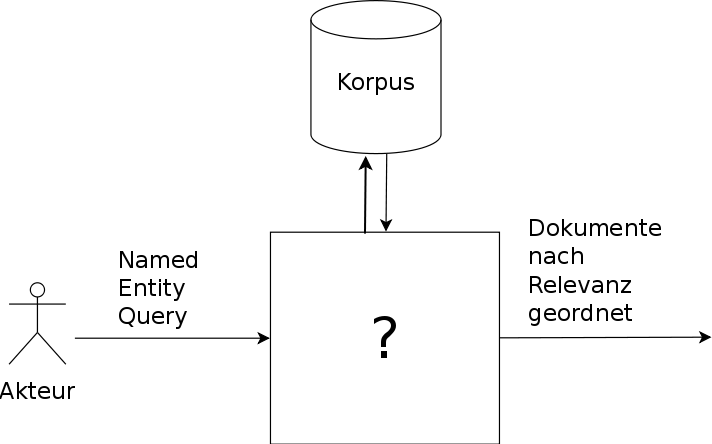
\includegraphics[scale=0.4]{bilder/overview}
		\caption{Ein- und Ausgabe-Schema}
		\label{pic:input-output}
	\end{figure}

\end{frame}
%\subsection{Häufigkeit der Anfragen}
%\begin{frame}
	%Falls keine tolle Grafik zu diesem Punkt exisitert, wird er nur in einem Nebensatz erwähnt
%
%Hier kommen noch genau Zahlen hin. Laut Vortrag letzten Donnerstag waren glaub 71\% der Anfragen einer Suchmachschine (deren Namen entweder nicht genannt wurde, oder ich schon wieder vergessen habe) Queries mit named entities.
%Für den Vortrag werden hier noch fundierte Zahlen mit Refernz eingefügt.
%
%\end{frame}


\begin{frame}{Begriffsklärung}
%noch zu verfeinern, definition wäre schön, sonst block
\begin{block}{Named Entity}
         Named Entities (Eigennamen) beziehen sich auf Personen und Dinge der realen Welt.
\end{block}
Wir unterscheiden im Folgenden Named Entities, die sich auf

\begin{itemize}
	\item{Personen}
	\item{Objekte}
\end{itemize}
beziehen.
\end{frame}



\begin{frame}{Begriffsklärung}

\begin{block}{named entitiy}
Personennamen als named entity
\end{block}


\begin{wrapfigure}{r}{100pt}
	\includegraphics[scale=0.5]{bilder/Peterchen}
	\caption{Peter Chen}
	\label{pic:Peter-Chen}
\end{wrapfigure}

\textbackground ``Dr. \textnamedentity Peter \textbackground Pin-Shan \textnamedentity Chen \textbackground (Chinese: \chin{陳品山}) is an American computer scientist and Professor of Computer Science at Louisiana State University, who is known for the development of Entity-Relationship Modeling in 1976.''
\cite{wiki:PeterChen}

\end{frame}


\begin{frame}{Begriffsklärung}

\begin{block}{named entitiy}
	Objektname als named entity
\end{block}

\begin{wrapfigure}{r}{100pt}
	\includegraphics[scale=0.2]{bilder/er}
	\caption{ER-Diagramm}
	\label{pic:er-diagramm}
\end{wrapfigure}

\textbackground ``Dr. Peter Pin-Shan Chen (Chinese: \chin{陳品山}) is an American computer scientist and Professor of Computer Science at Louisiana State University, who is known for the development of \textnamedentity Entity-Relationship Modeling \textbackground in 1976.'' 
\cite{wiki:PeterChen}



\end{frame}



%Anaphorik
\begin{frame}{Begriffsklärung}

	\begin{block}{Anaphorik}
		Bei einer anaphorischen Verbindung bezieht sich ein hinterer Satzteil auf einen Vorderen.
	\end{block}

	\textbackground ``\textnamedentity Chen \textbackground has received several awards in the fields of Information Technology. \textanapher $\underbrace{He}_{anaphoric\ expression}$ \textbackground received the Data Resource Management Technology Award[\ldots]''
	\cite{wiki:PeterChen}


\end{frame}

%Coreferenz
\begin{frame}{Begriffsklärung}

\begin{block}{Koreferenz}
	``Koreferenz liegt vor, wenn in einer Äußerung mit zwei verschiedenen sprachlichen Ausdrücken dasselbe bezeichnet wird.''
	\cite{wiki:Koreferenz}
\end{block}

%\begin{wrapfigure}{r}{100pt}
%	\includegraphics[scale=0.5]{bilder/Peterchen}
%\end{wrapfigure}

	\textbackground `` \textnamedentity Chen \textbackground has received several awards in the fields of Information Technology. \textanapher He \textbackground received the Data Resource Management Technology Award[\ldots]''
	\cite{wiki:PeterChen}

\end{frame}

\begin{frame}{Plausible Koreferenzen - feasible expressions}
	\begin{block}{$A_P$ - mögliche Koreferenzen zu Personen}
		${he, she, his, her, himself, herself}$
	\end{block}
	\begin{exampleblock}{$A_P$}
		\textnamedentity Peter Chen \textbackground is cool. \textanapher He \textbackground is \ldots
	\end{exampleblock}
	\begin{block}{$A_O$}
		${it, its, \ldots}$
	\end{block}
	\begin{exampleblock}{$A_O$}
		\textnamedentity Big Bang Theory \textbackground is a series. \textanapher It \textbackground is well known in the US. \textanapher The series \textbackground is not known\ldots
	\end{exampleblock}


\end{frame}




\begin{frame}{Problem mit Relevanzschätzung}

	\textbackground `` \textnamedentity Chen \textbackground has received several awards in the fields of Information Technology. \textanapher He \textbackground received the Data Resource Management Technology Award [\ldots]''
	\cite{wiki:PeterChen}
	\\
	By the way,
	\\
	``\textnamedentity Knuth \textbackground was born in Milwaukee, Wisconsin, where \textanapher his \textbackground father owned a small printing business and taught bookkeeping at Milwaukee Lutheran High School, which \textanapher he \textbackground attended. \textanapher He \textbackground was an excellent student [\ldots]''
	\cite{wiki:DonaldKnuth}


\end{frame}


\begin{frame}{Problem mit Relevanzschätzung}
	Oft werden die Häufigkeiten der Entitäten unterschätzt, da die Entitäten selbst oder Koreferenzen nicht beachtet werden. Man muss sich also Kümmern um das:
	  \begin{itemize}
		  \item Erkennen der Entitäten
		  \item Erkennen der möglichen Koreferenzen
		  \item Richtiges zuordnen der Koreferenzen
	  \end{itemize}


\end{frame}


\begin{frame}{Problem mit Relevanzschätzung}
	Generell gibt es zwei Möglichkeiten:
	\begin{itemize}
		\item Das vollständige Auflösen der Koreferenzen
		\item Das hier vorgestellte statistische ad-hoc Verfahren
	\end{itemize}

\end{frame}




\section{Problemlösung mittels statistischem Ansatz}

\subsection{Annahme}
\begin{frame}
	\begin{block}{Basic assumption}
		``Our key assumption is that the frequency of anaphoric expressions is distributed over named entities in a document according to the probabilities of whether the document is elite for the named entities.''
		\cite{paper:NaNg}
	\end{block}
	\textbackground `` \textnamedentity Chen \textbackground has received several awards in the fields of Information Technology. \textanapher He \textbackground received the Data Resource Management Technology Award [\ldots]''
	\cite{wiki:PeterChen}
	\\
	By the way,
	\\
	\textbackground ``\textnamedentity Knuth \textbackground was born in Milwaukee, Wisconsin, where \textanapher his \textbackground father owned a small printing business and taught bookkeeping at Milwaukee Lutheran High School, which \textanapher he \textbackground attended. \textanapher He \textbackground was an excellent student [\ldots]``
	\cite{wiki:DonaldKnuth}


\end{frame}



\begin{frame}{Flussdiagramm - Schritte um eine statistische Auflösung des Problems zu erhalten}

	\begin{figure}
		\includegraphics[scale=0.3]{bilder/h-overview}
		\caption{Ein- und Ausgabe-Schema}
		\label{pic:h-overview}
	\end{figure}
\end{frame}

\begin{frame}{Erkennen des Entity-Typs}
Da wir verschiedene anaphorische Ausdrücke für Personen und Objekte haben, wird zunächst bestimmt, ob die Entität eine Person oder ein Objekt ist.\\
\begin{itemize}
\item $A_P$ = \{he,she,his,her,himself,herself (who,whome)\}
\item $A_O$ = \{it,its\}
	\[ f_P(Q) = \frac{1}{|F(Q)|} \sum_{d \in F(Q)} \frac{tf(A_P;d)}{len(d)}\]

	\[ f_O(Q) = \frac{1}{|F(Q)|} \sum_{d \in F(Q)} \frac{tf(A_O;d)}{len(d)}\]
\end{itemize}
\end{frame}

\begin{frame}{Erkennen des Entity-Typs}

	\begin{figure}
		\includegraphics[scale=0.4]{bilder/Diskriminanzfunktion}
		\caption{Abbildung einer Hyperebene durch eine SVN \cite{wiki:svn}}
		\label{pic:Diskriminanzfunktion}
	\end{figure}

\end{frame}


\subsection{Feedback-based identification of anaphoric expressions}

\begin{frame}{Schritte für die Feedback-based identification}
Die feedback based Identifikation wird in 5 Schritten ausgeführt.
\begin{itemize}
	\item Erzeuge lexiko-syntaktische Muster
	\item Extrahieren der M relevantesten Dokumenten
	\item head-nouns extrahieren
	\item bestimme $tf(\text{head-noun};d)$
	\item filtern
\end{itemize}
\end{frame}

\begin{frame}{FB-I: 1.Schritt}
	query = ``Brokeback Mountain''
	\begin{exampleblock}{simple noun-phrase}
		\begin{itemize}
			\item the film
			\item the NN
		\end{itemize}
	\end{exampleblock}
	\begin{exampleblock}{more sophisticated noun-phrase}
		\begin{itemize}
			\item the fantastic film
			\item the JJ NN
		\end{itemize}
	\end{exampleblock}
\end{frame}

\begin{frame}{FB-I: 2.Schritt}
	Dann werden die M relevantesten Dokumente gesucht.
	\[BM25(e_Q;d)=OkapiTF(e_Q;d)\cdot IDF(e_Q;d)\]

	\[OkapiTF(e_Q;d)=\frac{(k_1+1)\cdot tf(e_Q;d)}{tf(e_Q;d)+k_1\left( (1-b)+b\frac{len(d)}{avglen(d)} \right)}\]

\end{frame}

\begin{frame}{FB-I: 3.Schritt - Extrahiere die head-nouns}
	\begin{table}
		\centering
		\begin{tabular}{lrlr}
			\toprule
			\multicolumn{2}{c}{\textbf{Q872:} ``Brokeback Mountain''} & \multicolumn{2}{c}{\textbf{Q1048:} ``Sopranos''} \\
			\midrule
			Head-noun & Frequency & Head-noun & Frequency \\
			film	& 85	& show & 29 \\
			movie & 59 & season & 16 \\
			story & 44 & series & 13 \\
			line & 31 & bracco & 13 \\
			year & 21 & cents & 8 \\
			audience & 21 & graduate & 8 \\
			world & 19 & time & 7\\
			\bottomrule
		\end{tabular}
		\caption{Top head-nouns sorted by their frequencies in the top 50 documents, for Q872 and Q1048}
		\cite{paper:NaNg}
	\end{table}
\end{frame}

\begin{frame}{FB-I: 4.Schritt}
	Die besten Treffer der Tabelle werden als anaphoric expressions angesehen.
\end{frame}


\begin{frame}{FB-I: 5.Schritt - Filter}
	\begin{table}
		\centering
		\begin{tabular}{lrlr}
			\toprule
			\multicolumn{2}{c}{\textbf{Q872:} ``Brokeback Mountain''} & \multicolumn{2}{c}{\textbf{Q1048:} ``Sopranos''} \\
			\midrule
			Head-noun & Frequency & Head-noun & Frequency \\
			film	& 85	& show & 29 \\
			movie & 59 & season & 16 \\
			story & 44 & series & 13 \\
			line & 31 & bracco & 13 \\
			\sout{year} & 21 & cents & 8 \\
			audience & 21 & graduate & 8 \\
			world & 19 & time & 7\\
			\bottomrule
		\end{tabular}
		\caption{Top head-nouns sorted by their frequencies in the top 50 documents, for Q872 and Q1048}
		\cite{paper:NaNg}
	\end{table}
\end{frame}


\section{Statistische Auswertung}

\subsection{Formalisierung}

\begin{frame}{True Entity Frequency}{Formelbeschreibung}
  % - A title should summarize the slide in an understandable fashion
  %   for anyone how does not follow everything on the slide itself.

  \begin{itemize}
	\item $Q$ = query (Suche)
	\item $e_Q$ = query entity (gesuchte Entität)
	\item $e_N$ = non-query entity
	\item $A$ = Menge plausibler anaphorischer Ausdrücke
	\item $tf(A;d)$ = Anzahl von $A$ in Dokument $d$
	\item $\varepsilon (A;d)$ = Menge plausibler Entitäten in Dokument $d$
	\item $tf(e;d)$ = raw entity frequency
	\item $atf(e;A,d)$ = anaphoric entity frequency
  \end{itemize}
\end{frame}

\begin{frame}{True Entity Frequency}
\begin{itemize}
\item True Entity Frequency of $e_Q$:
	\[tf_{TRUE}(e_Q;d) = tf(e_Q;d) + atf(e_Q;A,d)\]
\item Hauptproblem ist die Abschätzung von $atf(e_Q;A,d)$
\item Idee: Ignoriere den Kontext und multipliziere mit Faktor $P(e_Q|A,d)$
\item $P(e_Q|A,d):=$ Die Wahrscheinlichkeit, dass eine anaphoric expression sich auf die gesuchte Entität bezieht
\[ \Rightarrow tf_{TRUE}(e_Q;d) \approx tf(e_Q;d) + P(e_Q|A,d)tf(A;d)\]
\end{itemize}
\end{frame}


\subsection{Eliteness-Based Approximation}

\begin{frame}{Ist ein Dokument "elite" oder nicht?}
	\textbf{Definition: Eliteness}\cite{paper:NaNg} \\
\begin{quote}
"A document is \textbf{elite} for a term if the document is \underline{about} the concept represented by the term. [...] 
% In this paper, eliteness is used for multi-word named entities, in addition to single-word terms.
That is, a document is elite for a named entity if the document is about the entity." \footnote{A 2-Poisson model for probabilistic Coreference of Named Entities for Improved Text Retrieval -- Seung-Hoon Na; Hwee Tou Ng}
\end{quote}
\end{frame}

\begin{frame}{Ist ein Dokument "elite" oder nicht?}
\begin{itemize}
\item Definiere: $P(\textbf{E}(e)=1|d)$ als die Wahrscheinlichkeit, dass ein Dokument für eine Entität $e$ "elite" ist
\item Annahme: Die Bezüge der anaphoric expressions auf die Entitäten stehen im Zusammenhang, ob ein Dokument bzgl. dieser Entitäten "elite" ist oder nicht.
\[ \Rightarrow P(e_Q|A,d) = \frac{P(\textbf{E}(e_Q)=1|d)}{\sum_{e \in \varepsilon (A;d)}P(\textbf{E}(e)=1|d)} \]
\end{itemize}
\end{frame}

\begin{frame}{Vereinfachung der Formel}
\begin{itemize}
\item Sortiere alle non-query Entitäten nach der Wahrscheinlichkeit der Eliteness.
\item Selektiere die $K$ non-query Entitäten mit der höchsten Wahrscheinlichkeit.
\[ \Rightarrow P(e_Q|A,d) \approx \frac{P(\textbf{E}(e_Q)=1|d)}{P(\textbf{E}(e_Q)=1|d) + \sum_{i=1}^{K}P(\textbf{E}(e_N^{(i)})=1|d)} \]
\item Suche eine repräsentative non-query Entität heraus. Die Wahrscheinlichkeit der Eliteness aller anderen $K$ Entitäten wird mit dieser gleichgesetzt.
\[ \Rightarrow P(e_Q|A,d) \approx \frac{P(\textbf{E}(e_Q)=1|d)}{P(\textbf{E}(e_Q)=1|d) + K \cdot P(\textbf{E}(e_N)=1|d)} \]
\end{itemize}
\end{frame}

\subsection{Abschätzung der Eliteness}
\subsubsection{Threshold Model}

\begin{frame}{Threshold Model}
\begin{itemize}
\item Sehr einfaches und ungenaues Model
\item Annahme: Ein Dokument ist "elite" für Entität $e$, wenn gilt: $tf(e;d) \geq t$
\[ P(\textbf{E}(e)=1|d) = \delta (tf(e;d) \geq t)\]
\item Nehmen wir an das Dokument ist für die Top $K$ Entitäten elite, dann gilt also:
\[ P(e_Q|A,d) \approx \frac{\delta (tf(e;d) \geq t)}{ \delta (tf(e;d) \geq t) + K} \]
\end{itemize}
\end{frame}

\subsubsection{2-Poisson Mixture Model}

\begin{frame}{2-Poisson Mixture Model}
Erinnerung Poisson Verteilung:\\
Die Poisson-Verteilung liefert Voraussagen über die Anzahl $(k)$ des Eintretens seltener, zufälliger und voneinander unabhängiger Ereignisse innerhalb eines bestimmten Intervalls, wenn aus vorangehender Beobachtung bereits bekannt ist, wie viele Ereignisse man im Mittel innerhalb dieses Intervalls erwartet $(\lambda)$
\[P(X=k)=\frac{\lambda^k e^{-\lambda}}{k!}\]

\end{frame}

\begin{frame}{2-Poisson Mixture Model}
\begin{itemize}
\item Wir unterscheiden wieder:
\begin{itemize}
\item Das Dokument ist elite: Mittelwert $\lambda_e$
\item Das Dokument ist nicht elite: Mittelwert $\mu_e$
\end{itemize}
\item $\Rightarrow$ Die Wahrscheinlichkeit dass $e$ $tf$ mal in einem Dokument auftaucht ist:
\[ P(tf) = \pi_e \frac{e^{-\lambda_e}\lambda_e^{tf}}{tf!} + (1-\pi_e)\frac{e^{-\mu_e}\mu_e^{tf}}{tf!}\]
Wobei $\pi_e$ zuvor bestimmte Wahrscheinlichkeit ist, ob ein Dokument elite für eine Entität $e$ ist.\\
\item Mit Hilfe dieser Formel können wir nun die gesuchte Wahrscheinlichkeit berechnen.
\[ \frac{\pi_e P(tf(e;d)|\textbf{E}(e)=1)}{\pi_e P(tf(e;d)|\textbf{E}(e)=1)+(1-\pi_e) P(tf(e;d)|\textbf{E}(e)=0)}\]

\end{itemize}
\end{frame}

\begin{frame}{2-Poisson Mixture Model}

Für ein Dokument, welches bzgl $e$ elite ist gilt also:
\[ P(tf(e;d)|\textbf{E}(e)=1) =  \pi_e \frac{e^{-\lambda_e}\lambda_e^{tf}}{tf!} + (1-\pi_e)\frac{e^{-\mu_e}\mu_e^{tf}}{tf!}\]
Setzen wir das ein in:
\[ \frac{\pi_e P(tf(e;d)|\textbf{E}(e)=1)}{\pi_e P(tf(e;d)|\textbf{E}(e)=1)+(1-\pi_e) P(tf(e;d)|\textbf{E}(e)=0)}\]
erhalten wir:
\[ P(\textbf{E}(e) = 1|d) = \frac{\pi_e}{\pi_e + (1-\pi_e)e^{\lambda_e  \mu_e}\left( \frac{\mu_e}{\lambda_e}\right)^{tf(e;d)}}\]
\end{frame}

\begin{frame}{2-Poisson Mixture Model}{Bestimmen von $\lambda_e,\mu_e$ und $\pi_e$}
Unterscheide 2 Fälle:
\begin{itemize}
\item $e=e_Q$
\item $e \neq e_Q$
\end{itemize}
Sei nun $e=e_Q$\\
Annahme:
\begin{enumerate}
\item d ist elite $\Leftrightarrow tf(e;d) \geq 1$
\item Alle anderen Dokumente im Test sind non-elite bzgl. $e$
\end{enumerate}

\end{frame}

\begin{frame}
Dann gilt:
\[ \pi_e = \frac{df(e)}{df(e)+N}, \lambda_e = \frac{cf(e)}{df(e)}, \mu_e = \frac{cf(e)}{N}\]
\begin{itemize}
	\item $N$: Anzahl der Dokumente
	\item $df(e)$: Anzahl der Dokumente, in denen $e$ vorkommt
	\item $cf(e)$: Anzahl von $e$ in allen Dokumenten
\end{itemize}
Setzen wir das ein erhalten wir:
\begin{eqnarray*}
P(\textbf{E}(e) = 1|d) &=& \frac{\pi_e}{\pi_e + (1-\pi_e)e^{\lambda_e  \mu_e}\left( \frac{\mu_e}{\lambda_e}\right)^{tf(e;d)}}\\
	&=& \frac{1}{1+ \left( \frac{df(e)}{N}\right)^{tf(e;d)-1}e^{\frac{cf(e)}{df(e)}-\frac{cf(e)}{N}}}
\end{eqnarray*}

\end{frame}

\begin{frame}
Sei nun $e \neq e_Q$\\
Annahme:
\begin{enumerate} 
\item Alle non-query Entitäten sind vom selben Typ, wie die gesuchte Entität.
\item Die "Term Frequency" einer Top-$K$ non-query Entität ist gleich dem Durchschnittsvorkommen einer query Entität in einem elite Dokument
\end{enumerate}
Dann gilt also wieder:
\[ \pi_e = \frac{df(e)}{df(e)+N}, \lambda_e = \frac{cf(e)}{df(e)}, \mu_e = \frac{cf(e)}{N}\]
Setzen wir das ein erhalten wir:
\begin{eqnarray*}
P(\textbf{E}(e) = 1|d) &=&  \frac{1}{1+ \left( \frac{df(e)}{N}\right)^{\frac{cf(e)}{df(e)}-1}e^{\frac{cf(e)}{df(e)}-\frac{cf(e)}{N}}}
\end{eqnarray*}

\end{frame}

\begin{frame}{Eliteness Based Approximation}
Letztendlich können wir die berechneten Wahrscheinlichkeiten einsetzen in:
\[ \Rightarrow P(e_Q|A,d) \approx \frac{P(\textbf{E}(e_Q)=1|d)}{P(\textbf{E}(e_Q)=1|d) + K \cdot P(\textbf{E}(e_N)=1|d)} \]
Und dies in:
\[tf_{TRUE}(e_Q ; d) \approx tf(e_Q;d) + P(e_Q|A,d)tf(A;d)\]

\end{frame}

\begin{frame}{Eine allerletzte Verschönerung der Formel}
Um die term-frequency mit der Länge eines Dokumentes in Beziehung zu setzen, nutzen wir die \textit{normalized raw frequency}:
\[ntf(e;d) = \frac{tf(e;d) \cdot avglen}{len(d)}\]
Somit ist unsere geschätzte wahre term-freuqency definiert durch:
\[\boxed{ntf_{TRUE}(e_Q ; d) \approx ntf(e_Q;d) + P(e_Q|A,d)ntf(A;d)}\]
\end{frame}

\section{Evaluation}

%#################################
%Das ist ja wohl so nicht richtig!
%#################################

%\begin{frame}{Evaluation}
%	Die Herren Na und Ng haben festgestellt, dass ihr statistischer Ansatz immer bessere Ergebnisse erziehlt, als die aufwendige vollständige Auflösung der anaphorischen Ausdrücke.\\
%	Man beachte allerdings die klare Vereinfachung der Problemstellung.
%\end{frame}

\begin{frame}{Evaluation}
	\begin{itemize}
		\item Als Test-Set diente TREC blog '06, '07, '08
		\item entferne HTML-Tags und boiler templates
		\item für $BM25_{CEEF}(e_Q;d)$ verwende POS tagger
		\item für $SIM_{BASE}(Q;d)$ entferne stopwords und führe stemming aus
		\item Queries bestehen zu 95\% aus named entities ohne Kontext
		\item Beim Rest wurde der Kontext manuell entfernt
	\end{itemize}
	\begin{exampleblock}{query input}
	``Mark Warner \sout{for President}'' (Q1006) \cite{paper:NaNg}
\end{exampleblock}

\end{frame}

\begin{frame}{Evaluation - Training the Person Query Classifier}
	\begin{itemize}
		\item 50 Anfragen als training set
		\item Radial Basis Function berechnet Hyperebene
	\end{itemize}
	Ergebnis: 93\% Trefferquote

\end{frame}


%\begin{frame}{Evaluation - Baseline Runs} 
%	Die Baseline Runs wurden mit 
%	\begin{itemize}
%		\item bla
%	\end{itemize}
%
%\end{frame}

\begin{frame}{Evaluation}
	\begin{table}
		\centering
		\begin{tabular}{lS[tabnumalign=centre,tabformat=1.4,decimalsymbol=comma]S[tabnumalign=centre,tabformat=1.4,decimalsymbol=comma]S[tabnumalign=centre,tabformat=1.4,decimalsymbol=comma]}
			\toprule
			Methods & {MAP} & {Pr@5} & {Pr@10}\\
			\midrule
			REF & 0.3929 & 0.6707 & 0.6616\\
			CEEF-Thr & 0.3968 & 0.6788 & 0.6778\\
			CEEF-2Poisson & 0.4139 & 0.7060 & 0.6940\\
			CEEF-FB-2Poisson & 0.4165 & 0.7320 & 0.7200\\
			CEEF-FB-2Poisson* & 0.4177 & 0.7420 & 0.7270\\
			\bottomrule
		\end{tabular}
		\caption{Comparison of MAP, Pr@5, Pr@10}
		\cite{paper:NaNg}
	\end{table}


\end{frame}

\begin{frame}{Evaluation}
	\begin{table}
		\centering
		\begin{tabular}{lS[tabnumalign=centre,tabformat=1.4,decimalsymbol=comma]S[tabnumalign=centre,tabformat=1.4,decimalsymbol=comma]}
			\toprule
			Methods & {LM} & {LMFB} \\
			\midrule
			B (Baseline Run) & 0.4043 & 0.4254 \\
			B+REF & 0.4665 & 0.4868 \\
			B+CEEF-Thr & 0.4831 & 0.4942 \\
			B+CEEF-2Poisson & 0.4874 & 0.5000 \\
			B+CEEF-FB-2Poisson & 0.5074 & 0.5090 \\
			B+CEEF-FB-2Poisson* & 0.5087 & 0.5106 \\
			\bottomrule
		\end{tabular}
		\caption{Comparison of MAP of REF and CEEF methods combining with Language Models}
		\cite{paper:NaNg}
	\end{table}
\end{frame}


\begin{frame}{Evaluation}
\begin{table}
	\centering
		\begin{tabular}{lS[tabnumalign=centre,tabformat=1.4,decimalsymbol=comma]S[tabnumalign=centre,tabformat=1.4,decimalsymbol=comma]S[tabnumalign=centre,tabformat=1.4,decimalsymbol=comma]S[tabnumalign=centre,tabformat=1.4,decimalsymbol=comma]}
			\toprule
			Query Type & {REF} & {CEEF} & {CEEF-FB} & {CEEF-FB*}\\
			\midrule
			Person & 0.5640 & 0.5793 & 0.5761 & 0.5781\\
			Company, etc. & 0.5061 & 0.5170 & 0.5305 & 0.5305\\
			Product & 0.5245 & 0.5401 & 0.5680 & 0.5680\\
			TV program, etc & 0.3664 & 0.3754 & 0.3793 & 0.3994\\
			Organization & 0.4468 & 0.4682 & 0.4701 & 0.4701\\
			Event, etc. & 0.5039 & 0.4987 & 0.5012 & 0.5021\\
			Other Types & 0.4785 & 0.4889 & 0.5040 & 0.5040\\
			Topic & 0.2754 & 0.3078 & 0.3094 & 0.3123\\
			All & 0.4868 & 0.5000 & 0.5090 & 0.5106\\
			\bottomrule
		\end{tabular}
		\caption{Comparison of MAP of REF and CEEF methods, combining with LMFB each query type.\cite{paper:NaNg}}
\end{table}

\end{frame}

\begin{frame}{Evaluation}

	\begin{table}
		\centering
		\begin{tabular}{lS[tabnumalign=centre,tabformat=1.4,decimalsymbol=comma]S[tabnumalign=centre,tabformat=1.4,decimalsymbol=comma]S[tabnumalign=centre,tabformat=1.4,decimalsymbol=comma]S[tabnumalign=centre,tabformat=1.4,decimalsymbol=comma]}
			\toprule
			Query Type & {NONE} & {REF} & {CEEF} & {CEEF-FB}\\
			\midrule
			TREC '07 & 0.5406 & 0.5569 & 0.5646 & 0.5733\\
			TREC '08 & 0.5032 & 0.5216 & 0.5248 & 0.5330\\
			\bottomrule
		\end{tabular}
		\caption{Comparison of MAP of TREC08BEST and others. NONE means non-combined baseline run.}
		\cite{paper:NaNg}
	\end{table}
\end{frame}



\begin{frame}{Kritik am Verfahren}
	\begin{itemize}
		\item Es werden nicht alle anaphorischen Ausdrücke berücksichtig
		\item Verfälschung des Wahrscheinlichkeitmultiplikators durch Vernachlässigung aller nicht-top-K Entitäten
		\item Poisson-Verfahren auch nur eine Näherung
		\item Events und TV werden nicht richtig erkannt
		\item Die Dokumente für den Test wurden stark angepasst (Kontextentfernung bei named entities)
	\end{itemize}
\end{frame}

%\begin{frame}{Kritik an der Evaluation}
%	\begin{itemize}
%		\item Der Leser wird nicht aufgeklärt, wie schnell das Verfahren nun wirklich ist
%		\item Es wird nicht näher ausgeführt, wieviele Koreferenzen nun wirklich richtig abgeschätzt wurden
%	\end{itemize}
%\end{frame}

\section*{Summary}

\begin{frame}{Summary}

  % Keep the summary *very short*.
  \begin{itemize}
  \item
    Für eine gute Term-Frequency-Schätzung ist es naheliegend, die Häufigkeit von \alert{Koreferenzen} mit in Betracht zu ziehen.
  \item
    Der \alert{statistische Ansatz} ist eine CPU-time schonende Variante mit guten Ergebnissen.
  \end{itemize}
  
%  % The following outlook is optional.
%  \vskip0pt plus.5fill
%  \begin{itemize}
%  \item
%    Outlook
%    \begin{itemize}
%    \item
%      Something you haven't solved.
%    \item
%      Something else you haven't solved.
%    \end{itemize}
%  \end{itemize}
\end{frame}



% All of the following is optional and typically not needed. 
\appendix
\section<presentation>*{\appendixname}
\subsection<presentation>*{For Further Reading}

\begin{frame}[allowframebreaks]
  \frametitle<presentation>{For Further Reading}
    
  \begin{thebibliography}{10}
    
  \beamertemplatebookbibitems
  % Start with overview books.


 
    
  \beamertemplatearticlebibitems
  % Followed by interesting articles. Keep the list short.
  \bibitem{paper:NaNg}
	Seung-Hoon Na, Hwee Tou Ng
	  \newblock{\em A 2-Poisson Model for Probabilistic Coreference of Named Entities for Improved Text Retrieval}


  \bibitem{wiki:PeterChen}
	  Modified: 21:02, 21 May 2010 Nineball
    \newblock {\em wikipedia}.
    \newblock {Date: 31.05.2010} 

  \bibitem{wiki:DonaldKnuth}
	    Modified: 15:46, 21 May 2010 AlanUS 
    \newblock {\em wikipedia}
    \newblock {Date: 03.06.2010}


  \bibitem{wiki:Koreferenz}
	  Korrigiert:  16:47, 17. Jul. 2009 Chriki
    \newblock {\em wikipedia}
    \newblock {Date: 03.06.2010}

  \bibitem{wiki:svn}
	  00:26, 13. Aug. 2007 ChristianBier 
	  \newblock {\em wikipedia}
    \newblock {Date: 03.06.2010}



  \end{thebibliography}
\end{frame}

\end{document}


